\documentclass[a4paper, twocolumn]{article}

\usepackage{pgfplots}
\pgfplotsset{width=\columnwidth, compat=newest} % 图片绘制的宽度是7cm,使用的pgfplots版本为1.13


\begin{document}

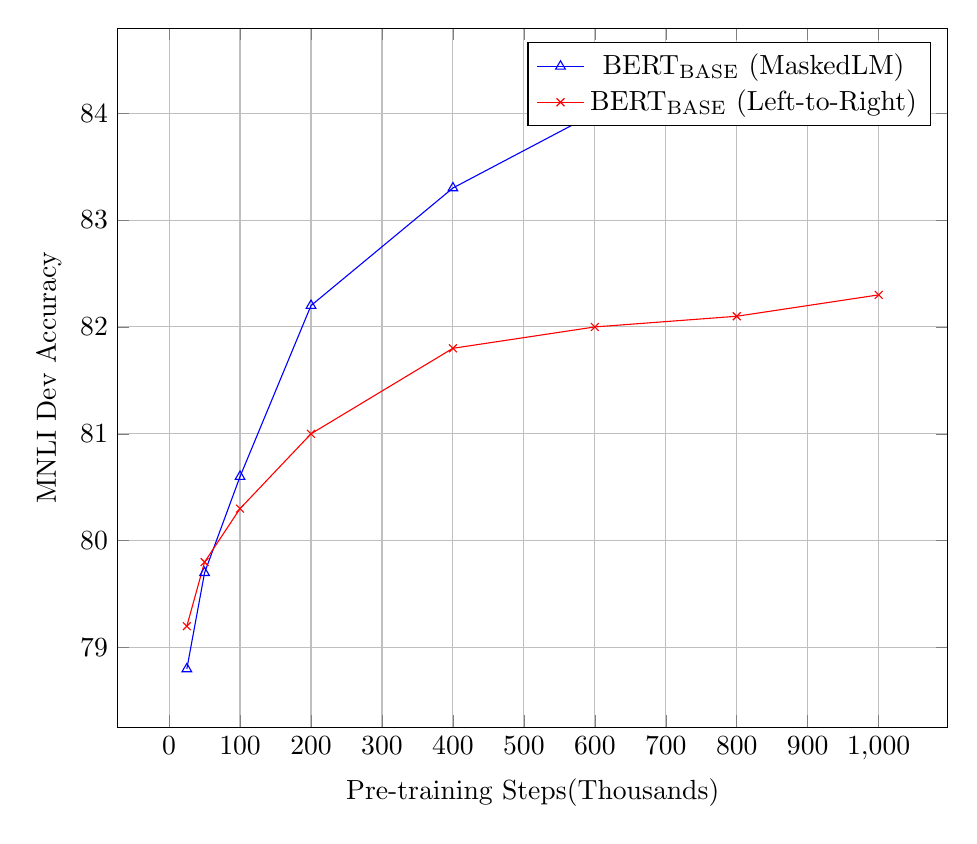
\begin{tikzpicture}
	\begin{axis}[
		xlabel=Pre-training Steps(Thousands),
		ylabel=MNLI Dev Accuracy,
		grid=major]

	\addplot[color=blue, mark=triangle] coordinates {
		(25, 78.8)
		(50, 79.7)
		(100, 80.6)
		(200, 82.2)
		(400, 83.3)
		(600, 84)
		(800, 84.15)
		(1000, 84.25)
	};
	\addlegendentry{$\rm BERT_{BASE}$ (MaskedLM)};
	
	\addplot[color=red,mark=x] coordinates {
		(25, 79.2)
		(50, 79.8)
		(100, 80.3)
		(200, 81)
		(400, 81.8)
		(600, 82)
		(800, 82.1)
		(1000, 82.3)
	};
	\addlegendentry{$\rm BERT_{BASE}$ (Left-to-Right)};
	
	\end{axis}
\end{tikzpicture}

\end{document}